%% Preamble %%
\documentclass[paper=a4]{article}

\usepackage{float}
\usepackage{geometry}
\geometry{verbose,tmargin=2.25cm,bmargin=2cm,lmargin=2.25cm,rmargin=2cm}
\geometry{a4paper}
\usepackage{multirow}


\usepackage[T1]{fontenc}
\usepackage{fourier}
\usepackage[utf8]{inputenc}
\usepackage[spanish]{babel}				

\usepackage{amsmath,amsfonts,amsthm} % Math packages

\usepackage{listings} % Pone el codigo lindo
\usepackage{color}

\definecolor{codegreen}{rgb}{0,0.6,0}
\definecolor{codegray}{rgb}{0.5,0.5,0.5}
\definecolor{codepurple}{rgb}{0.58,0,0.82}
\definecolor{backcolour}{rgb}{0.95,0.95,0.92}
 
\lstdefinestyle{mystyle}{
    backgroundcolor=\color{backcolour},   
    commentstyle=\color{codegreen},
    keywordstyle=\color{magenta},
    numberstyle=\tiny\color{codegray},
    stringstyle=\color{codepurple},
    basicstyle=\footnotesize,
    breakatwhitespace=false,         
    breaklines=true,                 
    captionpos=b,                    
    keepspaces=true,                 
    numbers=left,                    
    numbersep=5pt,                  
    showspaces=false,                
    showstringspaces=false,
    showtabs=false,                  
    tabsize=2
}
 
\lstset{style=mystyle}

\usepackage[pdftex]{graphicx}	

\makeatletter
%%%%%%%%%%%%%%%%%%%%%%%%%%%%%% User specified LaTeX commands.
\usepackage{fancyhdr}
\usepackage{lscape}
\pagestyle{fancy}
\lhead{Se\~nales Aleatorias 22.67}
\chead{TPL1}
\rhead{ITBA}
\renewcommand{\headrulewidth}{1pt}
\renewcommand{\footrulewidth}{1pt}

\makeatother

\usepackage{babel}
\addto\shorthandsspanish{\spanishdeactivate{~<>}}

\begin{document}

\tableofcontents
\newpage

\section{f.d.p. Gaussiana}

Para generar una f.d.p gaussiana $X$ con media $\mu_x$ y varianza $\sigma^2_x$, se utilizarán dos variables aleatorias $U_1$ y $U_2$ con distribución uniforme en (0,1).\par
Partiendo de dos variables aleatorias $R$ y $\Theta$, la función de distribución de $R$:

\[
F_R(r) = 1 - e^{-\frac{r^2}{2}} \hspace{2cm} 0<r<\infty
\]

Igualalndo a $U_1$ se puede despejar:

\[
F_R(r) = U_1 \Longrightarrow R = \sqrt{-2 \cdot \textrm{ln}(U_1)}
\]

La variable $\Theta$ tiene distribución uniforme:

\[
F_{\Theta}(\theta) = \frac{\theta}{2\pi} \hspace{2cm} 0<\theta<2\pi
\] 

Igualando a $U_2$ se despeja:

\[
F_{\Theta}(\theta) = U_2 \Longrightarrow \Theta = 2 \pi U_2
\]

Se tiene entonces que:

\[
Y = R \cdot \textrm{cos}(\Theta) \Longrightarrow Y = \sqrt{-2 \cdot \textrm{ln}(U_1)} \cdot \textrm{cos}(2 \pi U_2)
\]

Por lo que se consigue generar una variable aleatoria $Y\sim N(0,1)$. Para obtener la variable aleatoria $X$ con media y varianza personalizadas, se utiliza la transformación lineal:

\[
X = \sigma_x \cdot Y + \mu_x
\]
\par
Donde efectivamente:

\[
E(X) = \sigma_x \cdot \underbrace{E(Y)}_{=0} + \mu_x = \mu_x \hspace{2cm} \textrm{y} \hspace{2cm} \textrm{Var}(X) = \sigma^2_x \cdot \underbrace{\textrm{Var}(Y)}_{=1} = \sigma^2_x 
\]

\subsection{Estimación con $hist$, $mean$ y $std$}
Se realiz\'o la simulación utilizando vectores de 1000, 5000 y 50000 elementos, que permiten visualizar en forma clara la diferencia entre los histogramas y las curvas te\'oricas para cada caso, mostrando una corrida a continuación. En los histogramas se utilizaron 100 barras.\par
Los par\'ametros utilizados son $\mu_x = 3$ y $\sigma^2_x = 1$.

\begin{figure}[!ht]
\begin{centering}
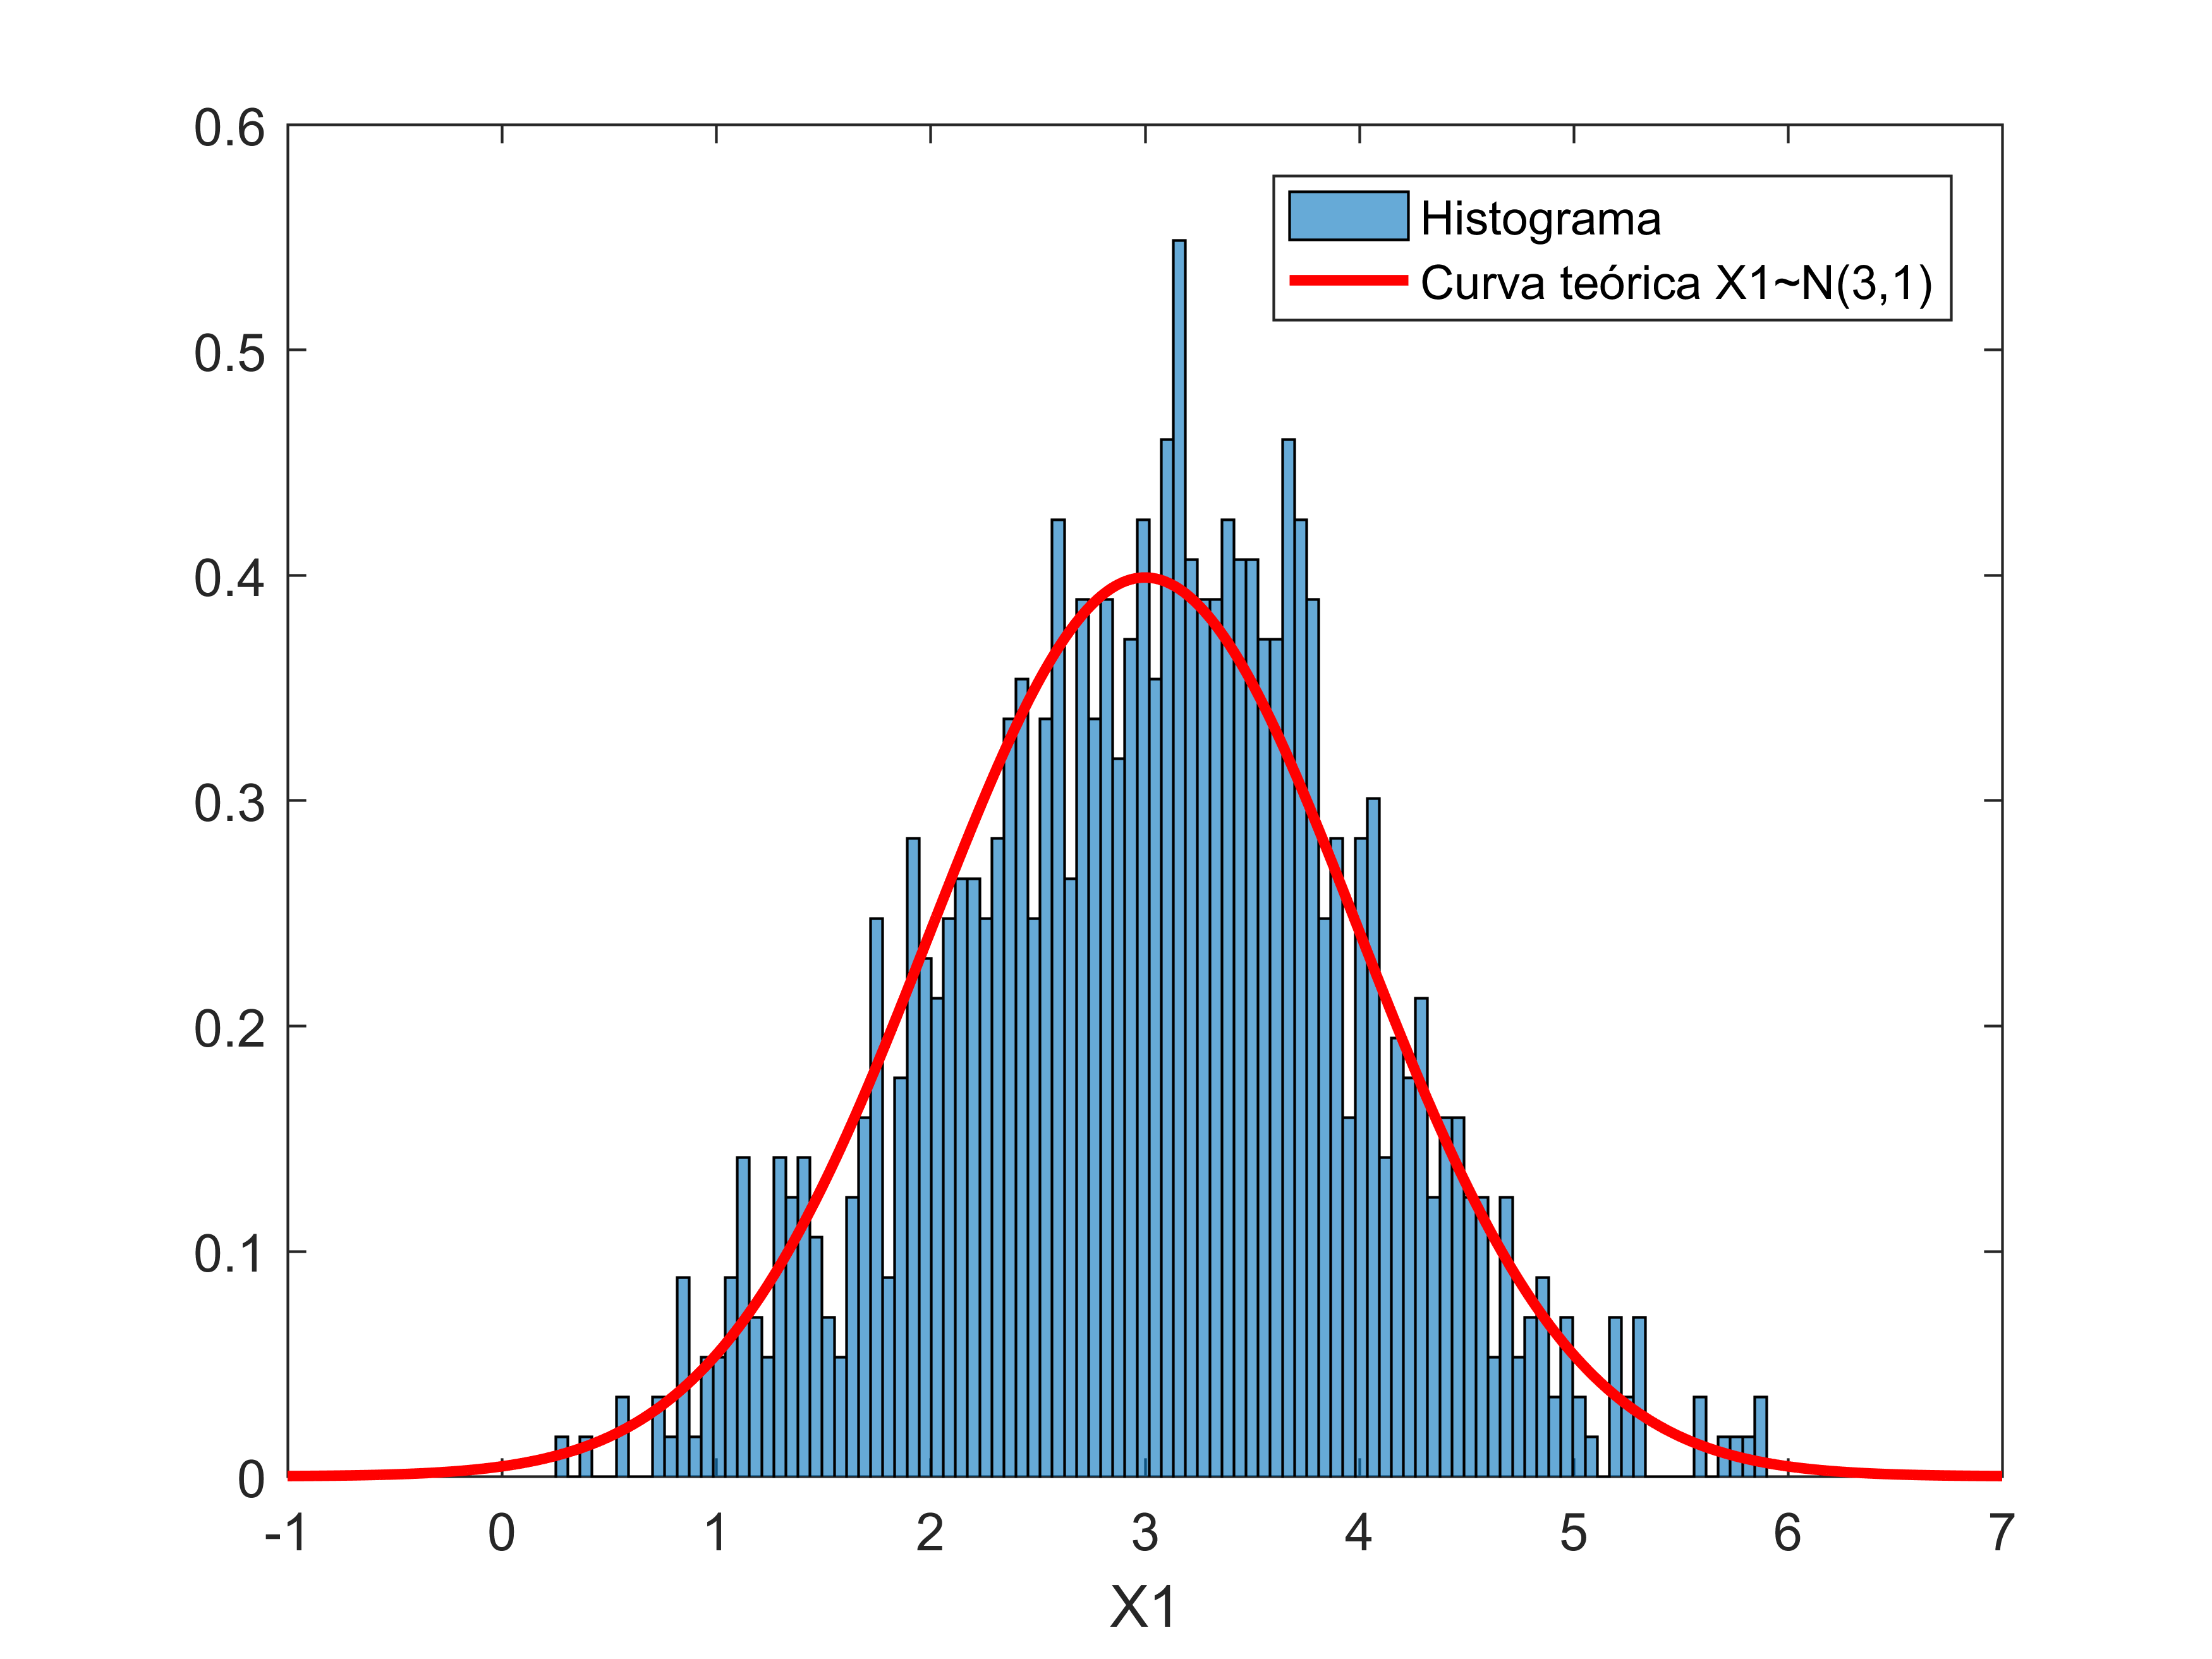
\includegraphics[scale=0.55]{Imagenes/X1_1000.png}
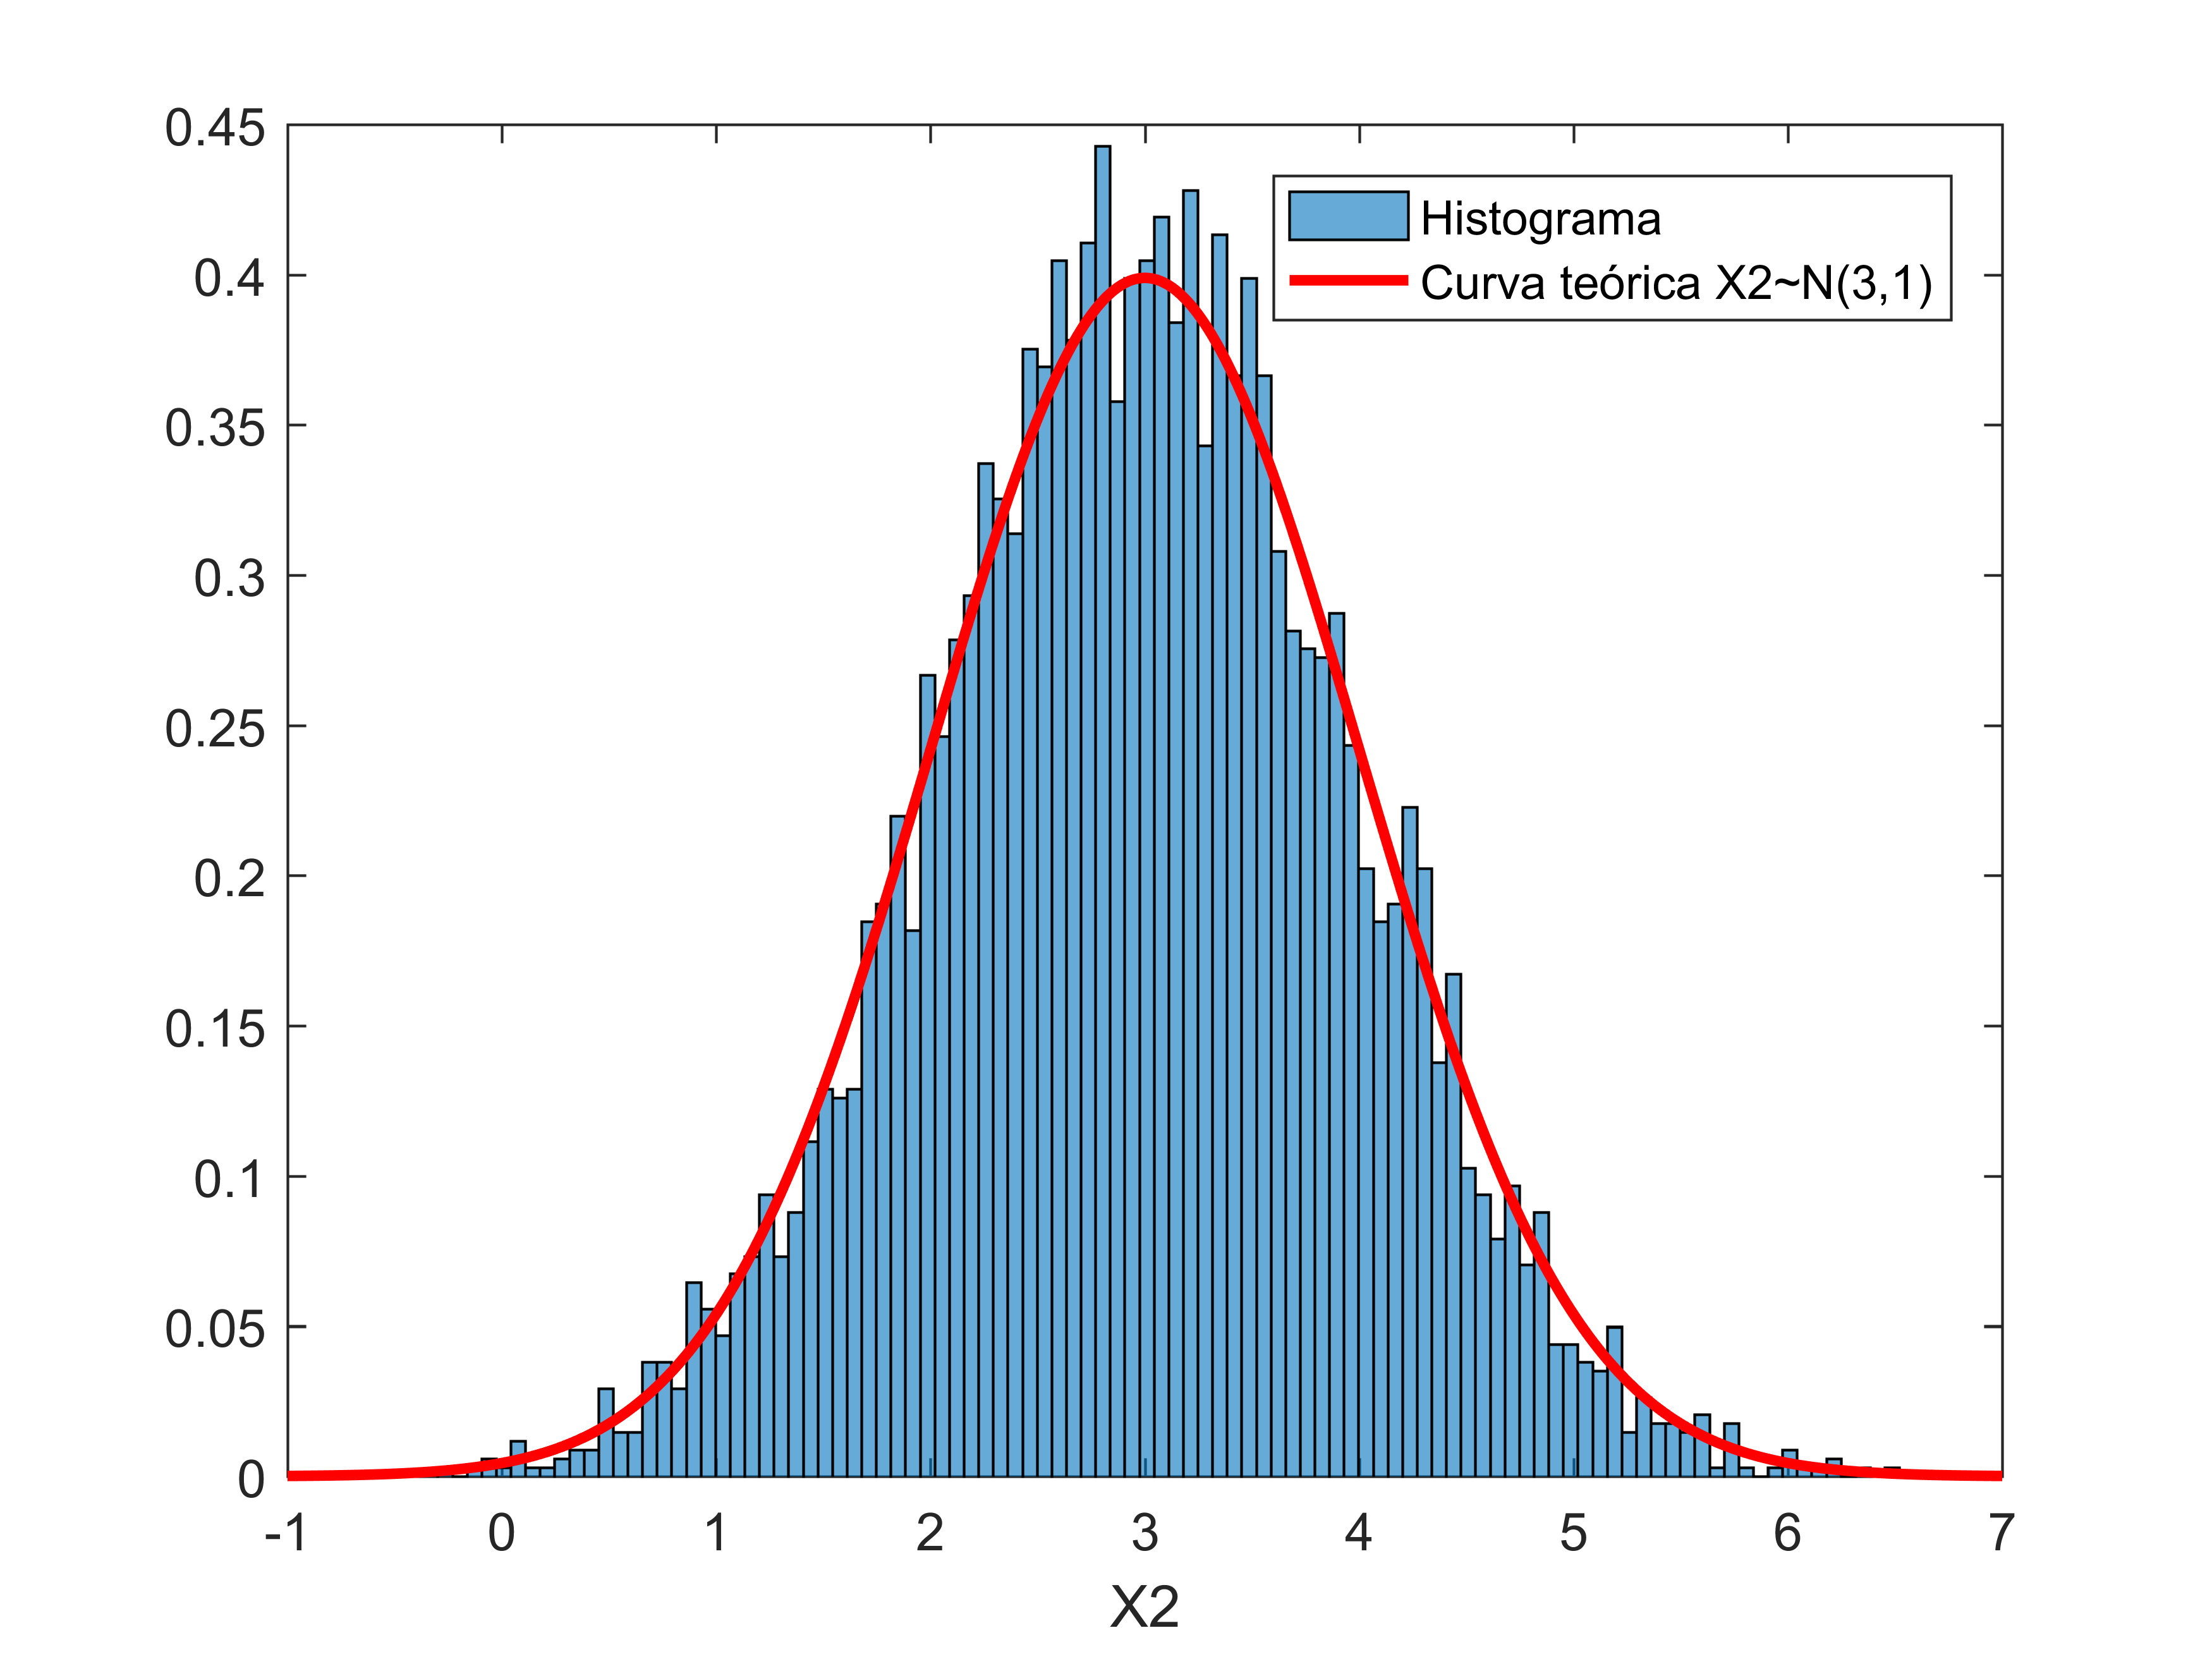
\includegraphics[scale=0.55]{Imagenes/X2_5000.png}
\par\end{centering}
\caption{Comparación para vectores $X_1$ de 1000 elementos e $X_2$ de 5000 elementos}

\end{figure} 

\newpage

\begin{figure}[!ht]
\begin{centering}
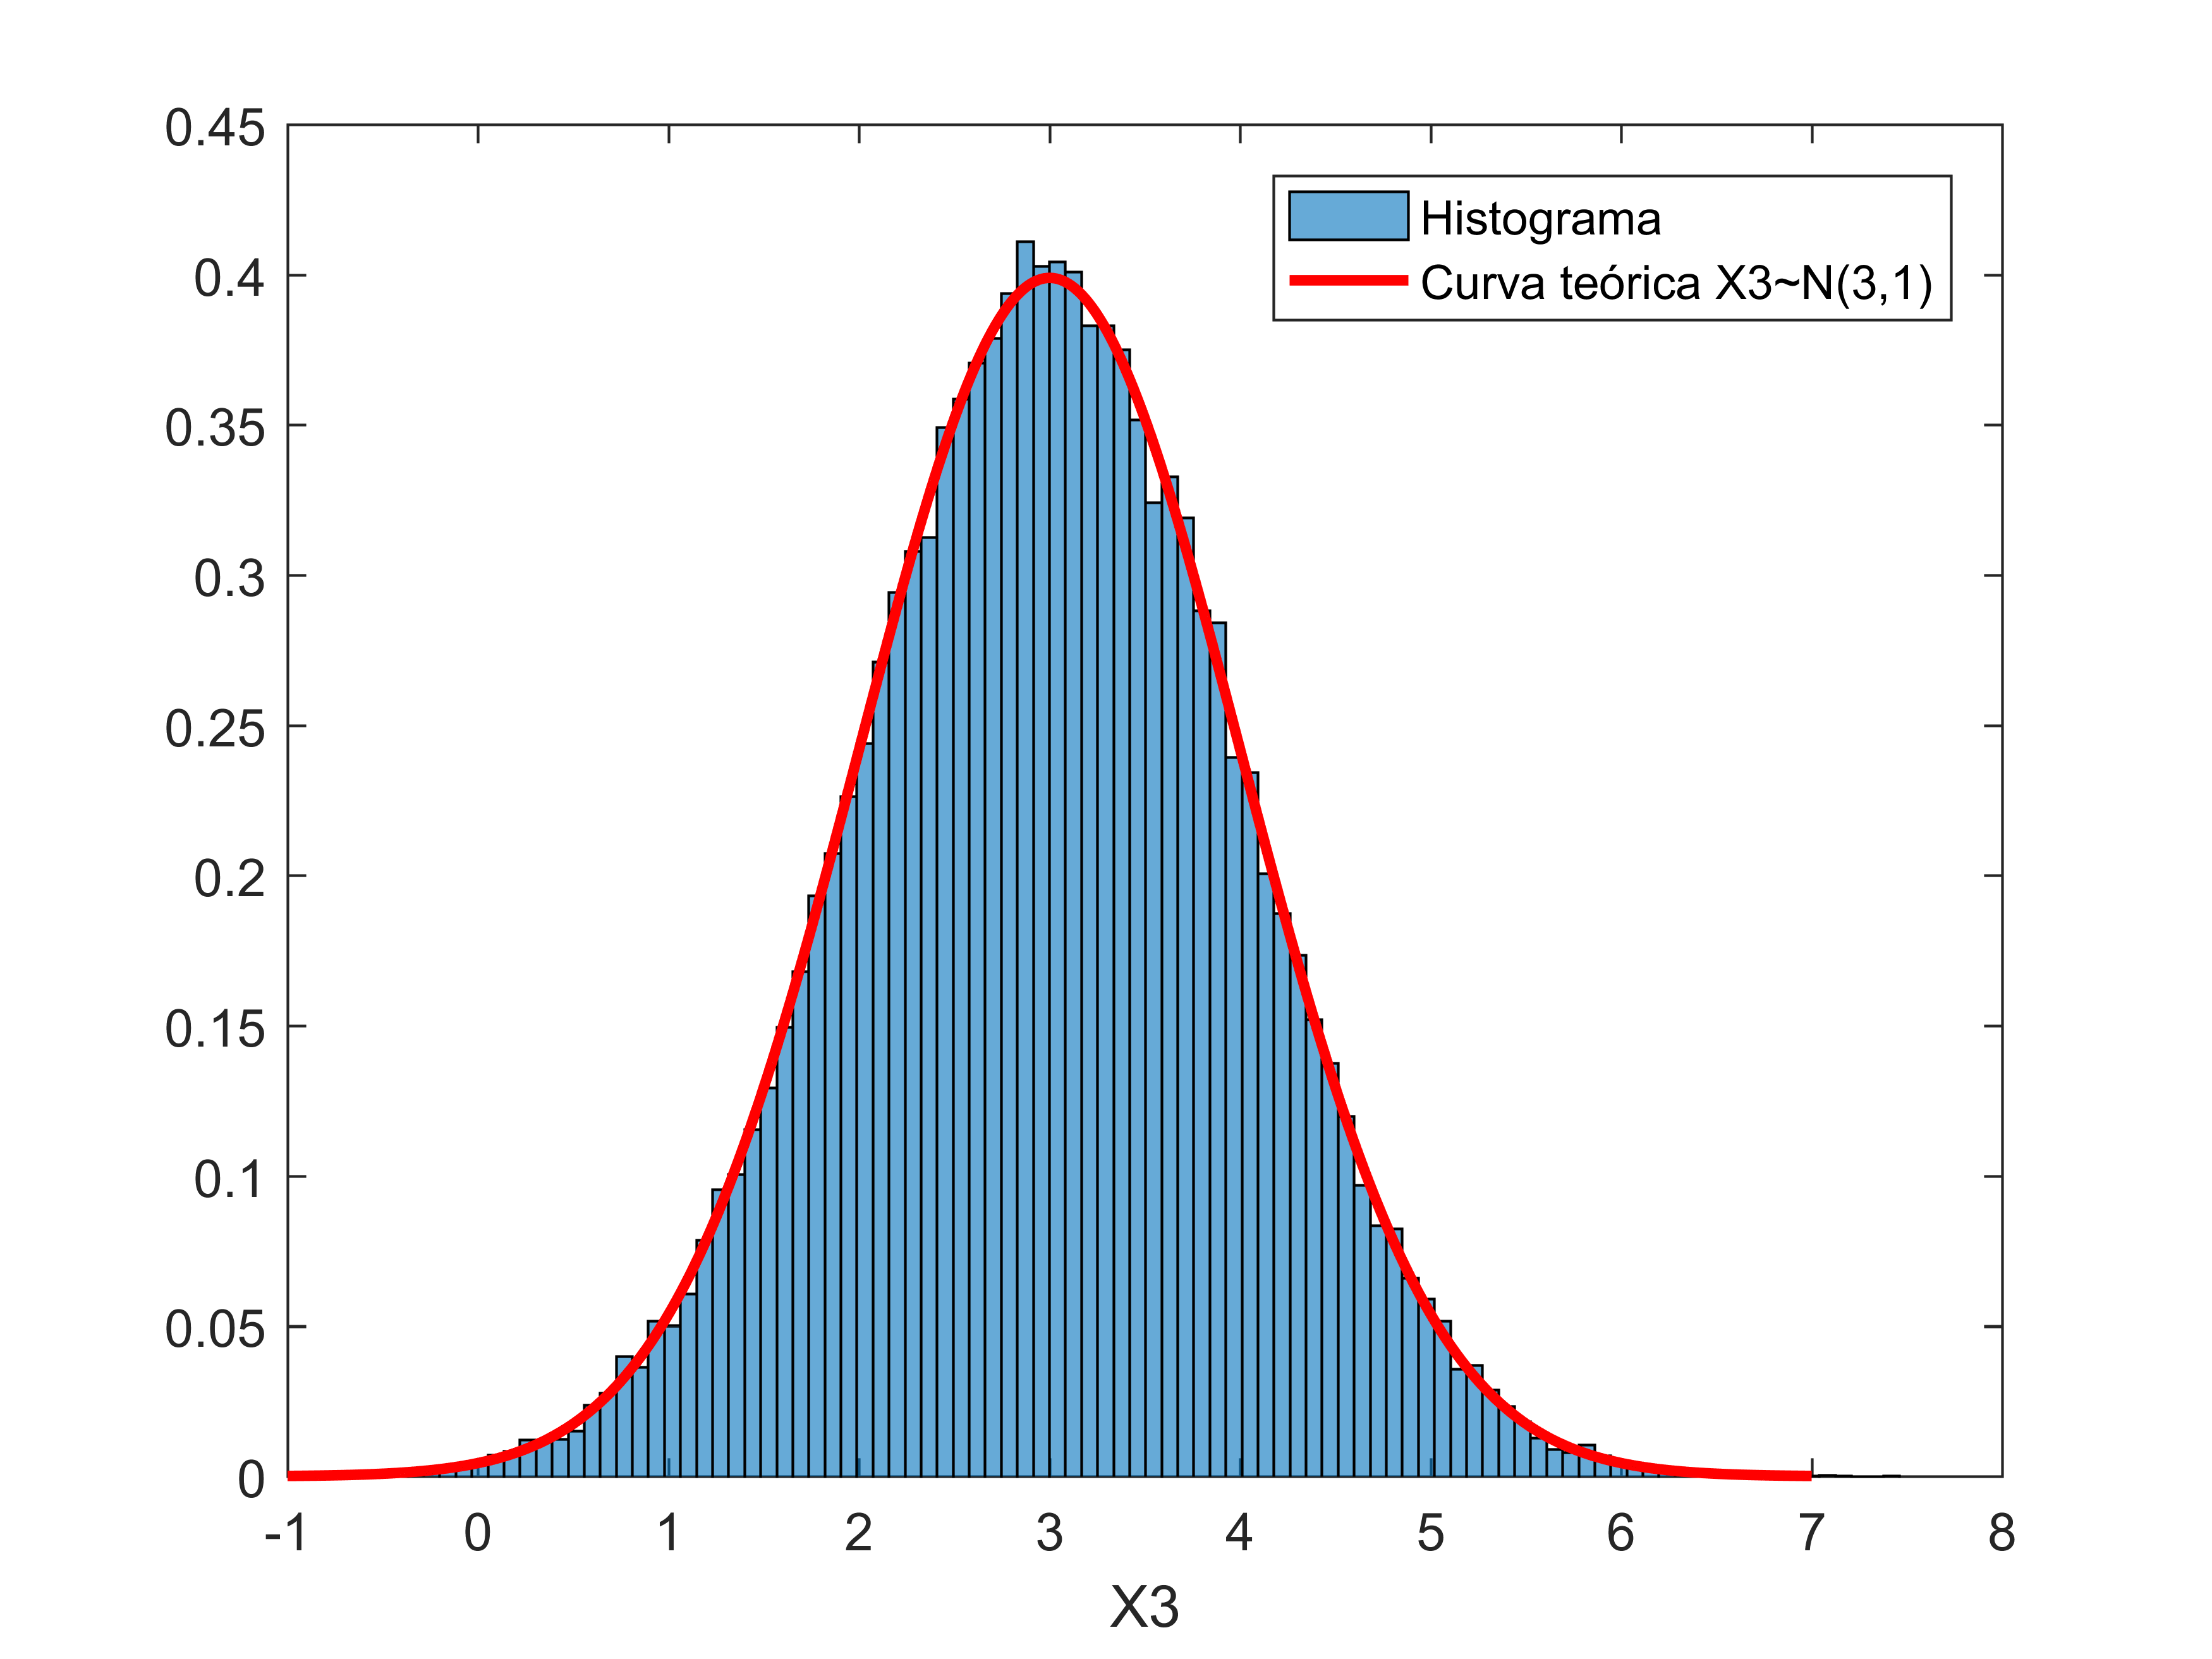
\includegraphics[scale=0.55]{Imagenes/X3_50000.png}
\par\end{centering}
\caption{Comparación para vector $X_3$ de 50000 elementos}

\end{figure} 

Utilizando un n\'umero fijo de barras adecuado, se consigue el ajuste mostrado en las gr\'aficas anteriores. Para mayor cantidad de elementos, el histograma tiende a parecerse m\'as a la curva de la gaussiana te\'orica.\par
El c\'odigo de MatLab utilizado para la simulaci\'on se muestra a continuaci\'on.

\lstinputlisting[language=Matlab, caption=Codigo de implementaci\'on]{Codigos/ItemAB.m}

\subsection{Valores de $\mu$ y $\sigma^2$ te\'oricas con estimadas}

De los vectores anteriores se estima la media y la varianza para cada caso, comparando con los te\'oricos en el siguiente cuadro.

\begin{table}[!ht]
\begin{centering}

\begin{tabular}{|c||c|c|c||c|c|c|}
\hline 
\multirow{2}{*}{Elementos} & \multicolumn{3}{c||}{$\mu_x$} & \multicolumn{3}{c|}{$\sigma^2_x$}\tabularnewline
\cline{2-7} 
 & Te\'orico & Estimado & $\Delta \mu_x$ & Te\'orico & Estimado & $\Delta \sigma^2_x$ \\
\hline 
\hline 
1000 & 3 & 3.0402 & 0.0402 & 1 & 0.9348 & 0.0652\\
\hline 
5000 & 3 & 2.9882 & 0.0118 & 1 & 0.9577 & 0.0423\\
\hline 
50000 & 3 & 3.0006 & 0.0006 & 1 & 0.9984 & 0.0016\\
\hline 
\end{tabular}
\par\end{centering}
\caption{Valores estimados y te\'oricos}

\end{table}

Dado que el n\'umero de elementos es bastante grande en los casos analizados, los valores estimados caen siempre muy cerca de los te\'oricos.

\subsection{Estimaciones de $\mu_x$ - Histograma}

Para este caso, se realizan 10000 estimaciones en distribuciones con 10000 elementos cada una. El c\'odigo de MatLab utilizado para la simulaci\'on es el siguiente.

\lstinputlisting[language=Matlab, caption=C\'odigo de implementaci\'on]{Codigos/ItemD.m}

\newpage

Realizando un histograma de los valores obtenidos, se tiene:

\begin{figure}[!ht]
\begin{centering}
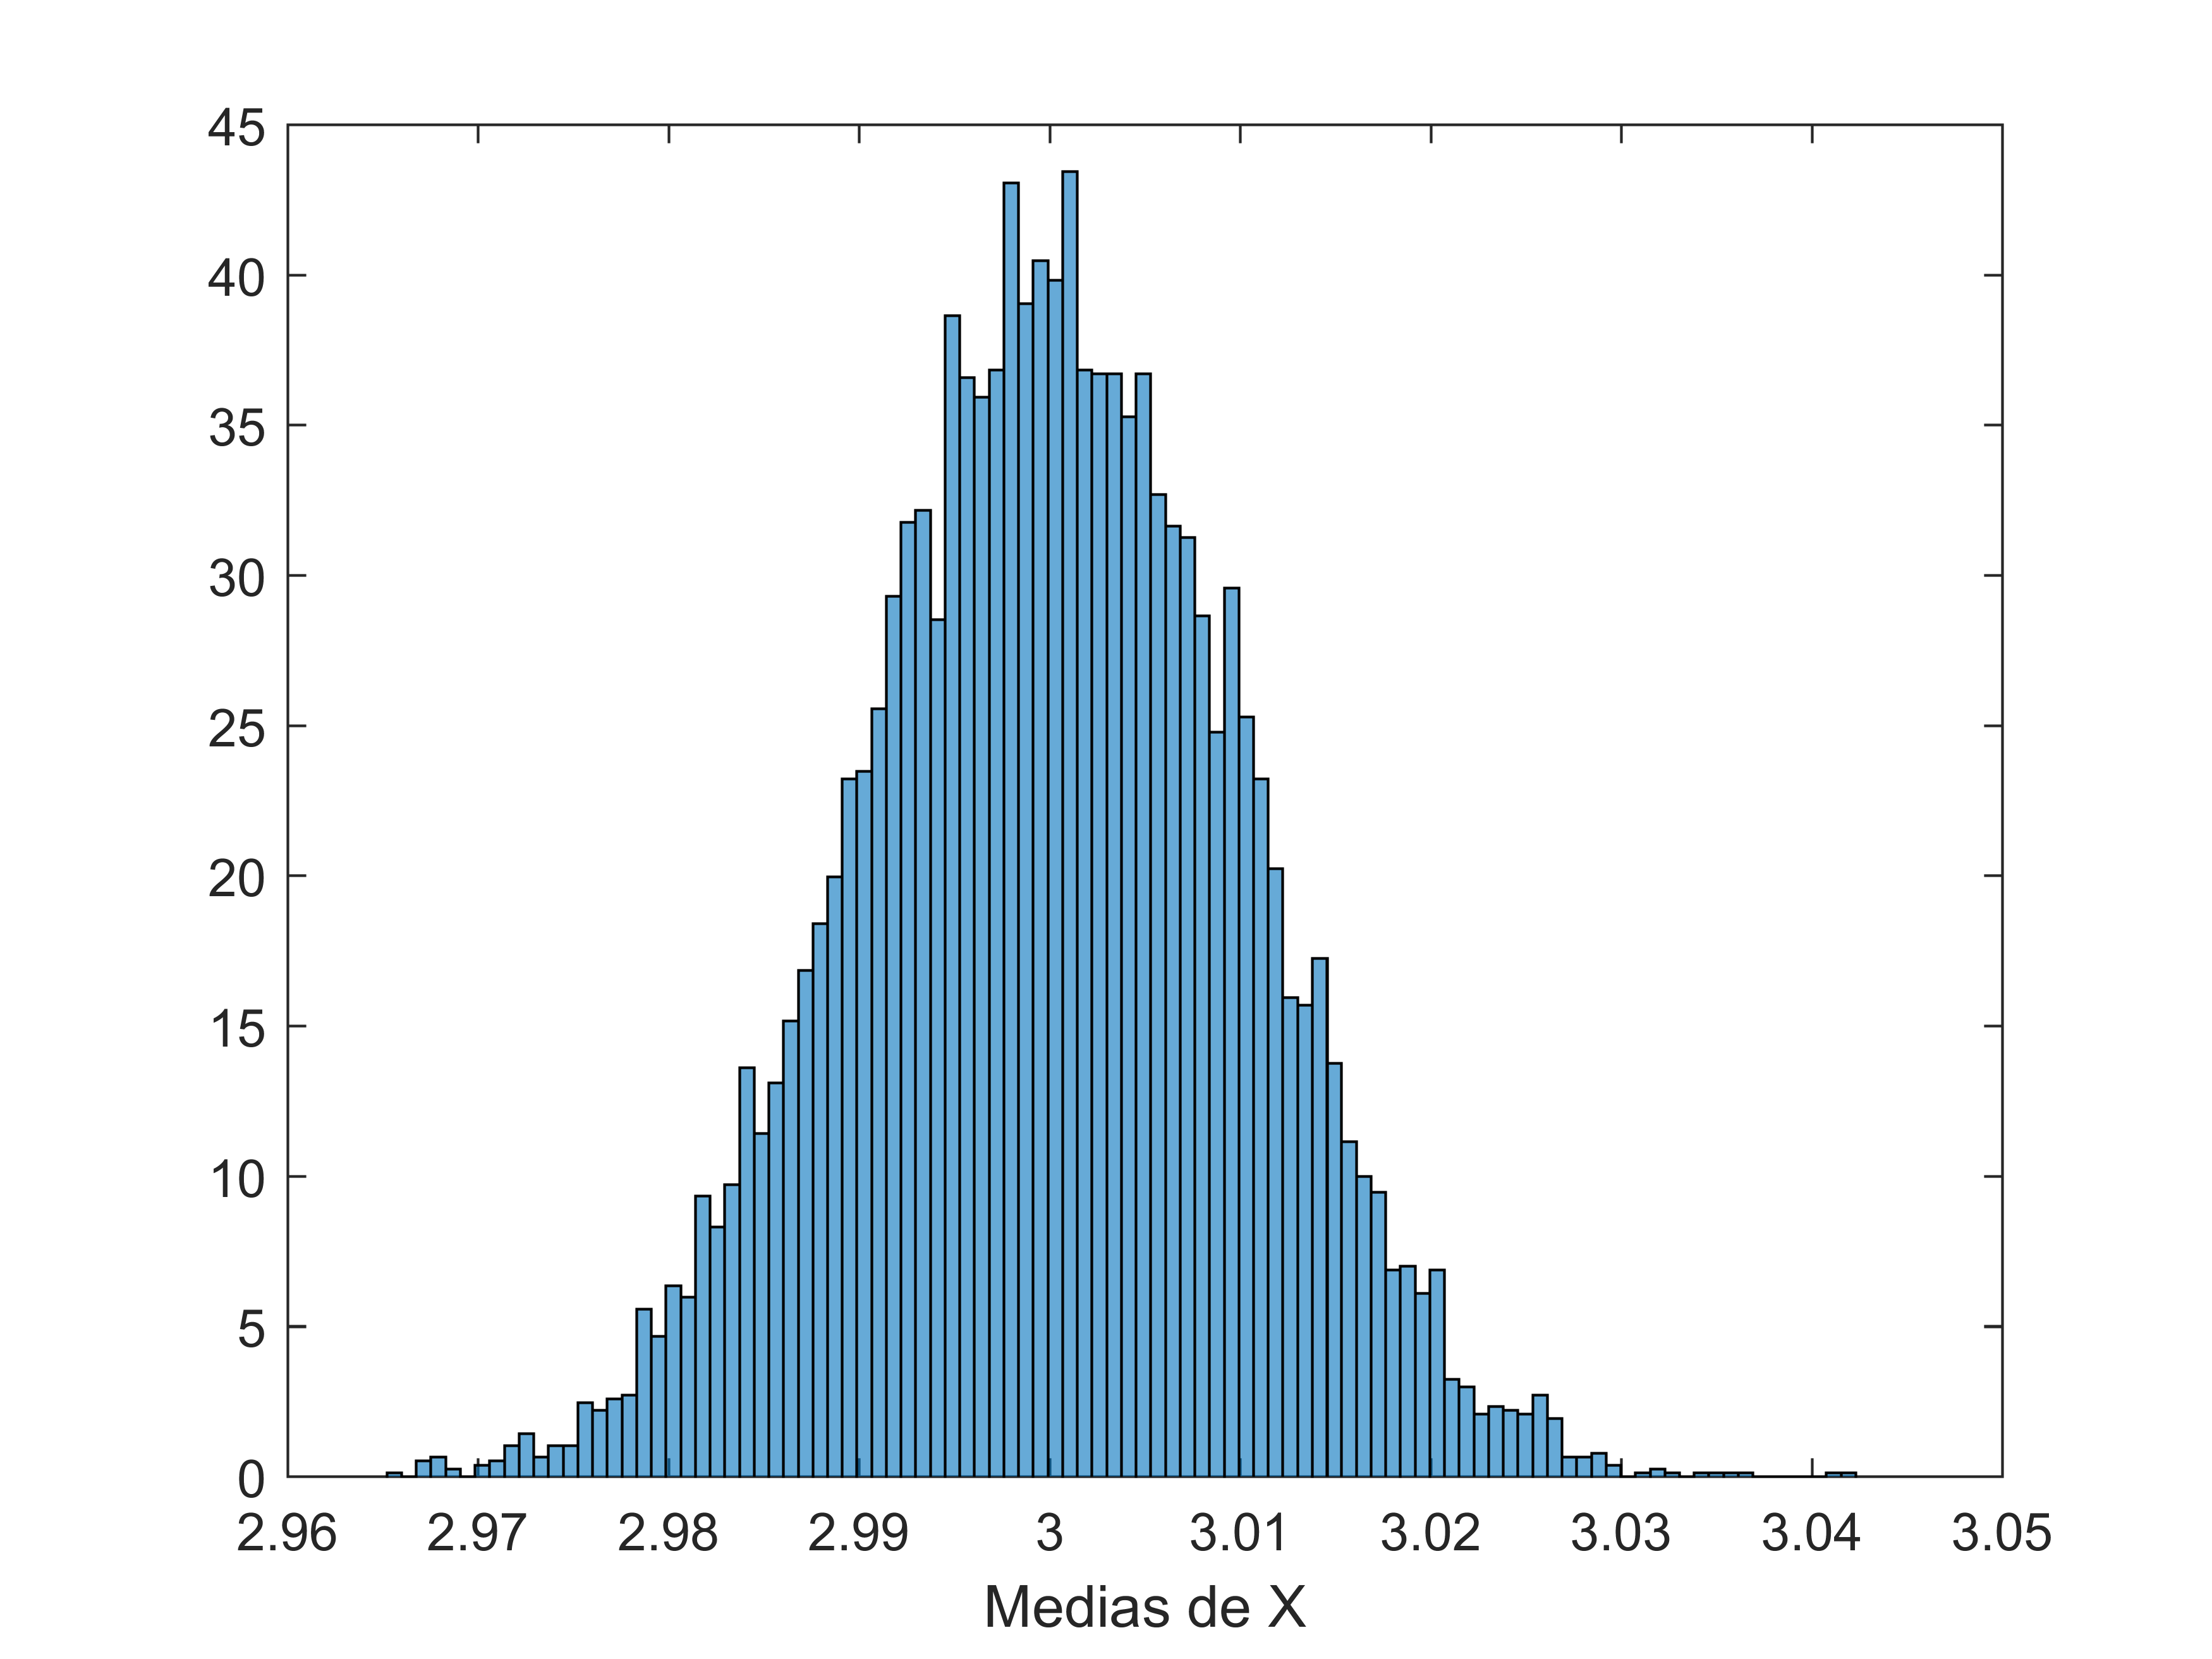
\includegraphics[scale=0.55]{Imagenes/MediasX.png}
\par\end{centering}
\caption{Histograma de las medias estimadas, con resultante $\mu = 3.0001$ - $\sigma = 0.01$}

\end{figure} 

Si llamamos a la media estimada $m_X$, se la define en este caso como:

\[
m_X = \frac{1}{N} \cdot \sum^N_{i=1} \mu_{X_i} \hspace{2cm} \textrm{Con N = 10000} 
\]

Como la distribuci\'on normal es reproductiva, la suma de N variables aleatorias con dicha distribuci\'on resulta tambi'en normal. Esto \'ultimo tambi\'en puede verse desde el Teorema Central del L\'imite, dado que el valor de N utilizado es suficientemente grande. Para el caso en cuesti\'on, los valores te\'oricos de $\mu$ y $\sigma$ son:

\[
E(m_X) = \mu = \frac{1}{N} \cdot \underbrace{\sum^N_{i=1} E(\mu_{X_i})}_{\textrm{Por linealidad}} = \frac{1}{N} \cdot \sum^N_{i=1} \mu_x = \mu_x \Longrightarrow \mu = 3
\]

\[
\sigma^2(m_X) = \sigma^2 = \frac{1}{N^2} \cdot \underbrace{\sum^N_{i=1} \sigma^2(\mu_{X_i})}_{\textrm{Por independencia}} = \frac{1}{N^2} \cdot \sum^N_{i=1} \sigma^2_x = \frac{\sigma^2_x}{N} \Longrightarrow \sigma = 0.0001
\]

De donde se observa que los valores estimados sobre la media del vector graficado en el histograma resultan muy cercanos a los te\'oricos.

\subsection{Error en la estimaci\'on de $\mu_x$ - Ejemplo}

Se toma ahora un caso particular, donde la cantidad de elementos es desconocida, y se busca que la probabilidad de que el valor estimado $m_X$ se aparte m\'as del 4\% del valor te\'orico sea menor al 2\%. Es decir:

\[
P[|m_X - \mu_x| > 0.04\mu_x] \leq 0.02
\]

Si se trabaja con la expresi\'on:

\[
2 \cdot P[m_X - \mu_x < -0.04\mu_x] \leq 0.02
\]
\[
P[\left( \frac{m_X - \mu_x}{\sigma_x} \right) \cdot \sqrt{N} < -0.04 \cdot \frac{\mu_x}{\sigma_x} \cdot \sqrt{N}] \leq 0.01
\]

La variable aleatoria $\left( \dfrac{m_X - \mu_x}{\sigma_x} \right) \cdot \sqrt{N}$ tiene distribuci\'on normal est\'andar. La llamamos $\Phi$:

\[
\Phi \left( -0.04 \cdot \frac{\mu_x}{\sigma_x} \cdot \sqrt{N} \right) \leq 0.01
\]
\[
\Phi \left( 0.04 \cdot \frac{\mu_x}{\sigma_x} \cdot \sqrt{N} \right) \geq 0.99
\]
\[
0.04 \cdot \frac{\mu_x}{\sigma_x} \cdot \sqrt{N} \geq \Phi^{-1}(0.99) \approx 2.3263
\]
\[
N \geq 3382.3 \cdot \frac{\sigma^2_x}{\mu^2_x}
\]

Para el caso analizado, $\mu_x = 3$ y $\sigma^2_x = 1$:

\[
N \geq 375.9
\]

El c\'odigo utilizado para verificar por simulaci\'on es el siguiente:

\lstinputlisting[language=Matlab, caption=C\'odigo de implementaci\'on]{Codigos/ItemE.m}

Donde la probabilidad P calculada efectivamente resulta $\leq 0.02$.

\section{Variables aleatorias conjuntamente gaussianas}

\section{Proceso de Poisson}

\end{document}